\chapter{Oszillatoren, Besetzungszahlen und das erste Quantenfeld}

Die Quantenfeldtheorie ist unser Rahmen für praktisch die gesamte bekannte nichtgravitative Physik. Diese Aussage darf nicht mit der Behauptung verwechselt werden, jedes Problem lasse sich lösen. Ein Wasserstoffatom ist noch handhabbar; bei einem Atom wie Bor wird die Rechnung bereits viel schwieriger, und ein Mensch liegt weit jenseits dessen, was sich mit einer realistischen feldtheoretischen Rechnung erfassen lässt. Der Rahmen mag fundamental sein, während seine Gleichungen überwältigend schwierig bleiben.

Wir nähern uns dem Thema daher auf die elementarste mögliche Weise. Das Gebiet wird manchmal als \emph{zweite Quantisierung} bezeichnet, doch der Name wird wenig bedeuten, bis wir den nötigen Formalismus aufgebaut haben. Der kürzeste Weg beginnt nicht mit einem relativistischen Feld, sondern mit dem harmonischen Oszillator. Federn sind nicht der entscheidende Punkt. Es geht um die Algebra der Erzeugungs- und Vernichtungsoperatoren. Wiederholt man diese Algebra für viele Moden, bedeutet ein Erzeugungsoperator nicht länger bloß ``einen Oszillator um eine Stufe anheben'', sondern ganz wörtlich ``ein Teilchen erzeugen.''

\section{Der Oszillator als Algebra}

Für einen einzelnen Oszillator sei \(a^\dagger\) der Operator, der die Anregung erhöht, und \(a\) derjenige, der sie erniedrigt. Die Schreibweisen \(a_+\) und \(a_-\) sind gleichwertig; die Dagger-Notation nimmt jedoch die in der Feldtheorie verwendete Sprache vorweg. Der Grundzustand erfüllt
\begin{equation}
a|0\rangle=0,
\end{equation}
und der Zahloperator ist
\begin{equation}
N=a^\dagger a,
\qquad
N|n\rangle=n|n\rangle.
\end{equation}
Die beiden Leiteroperatoren sind zueinander adjungiert, und ihr wesentlicher Kommutator lautet
\begin{equation}
[a,a^\dagger]=1.
\label{eq:l06-single-commutator}
\end{equation}
Diese kleine Algebra macht fast den ganzen Oszillator aus.

\(a\) und \(a^\dagger\) lassen sich als geeignete Linearkombinationen von Ort und Impuls darstellen. Die genaue Konvention hängt von der Normierung von \(x\), \(p\), \(m\) und \(\omega\) ab; die hier nützliche, von dieser Wahl unabhängige Aussage lautet, dass \(a^\dagger a\) den quadratischen Oszillator-Hamiltonoperator bis auf die additive Grundzustandsenergie rekonstruiert. Somit gilt
\begin{equation}
H=\hbar\omega\left(N+\frac12\right).
\end{equation}
Für die vorliegende Diskussion lassen wir den konstanten Term weg und verwenden
\begin{equation}
H=\hbar\omega N.
\label{eq:l06-one-oscillator-hamiltonian}
\end{equation}
Die Frequenz gibt an, welchen Preis eine Anregung hat. Eine Erhöhung von \(n\) um eins kostet \(\hbar\omega\); eine Erniedrigung von \(n\) um eins setzt denselben Betrag frei.

\section{Viele unabhängige Oszillatoren}

Betrachten wir nun viele Oszillatoren und kennzeichnen sie durch \(i\). Dieses Zeichen ist lediglich ein Index und nicht die imaginäre Einheit. Es kann endlich oder unendlich viele Moden geben. Eine Ansammlung unabhängiger Federn liefert ein Bild; die Normalmoden einer idealen Violinsaite ein anderes. Für die Anwendungen in der Feldtheorie ist der Fall mit unendlich vielen Moden entscheidend.

Unabhängigkeit hat eine operatorielle Bedeutung. Operatoren, die zu tatsächlich unabhängigen Teilsystemen gehören, kommutieren. Andernfalls könnten die zugehörigen Größen nicht unabhängig voneinander gemessen werden, und die Systeme wären von vornherein nicht unabhängig. Daher gilt
\begin{align}
[a_i,a_j]&=0, \\
[a_i^\dagger,a_j^\dagger]&=0, \\
[a_i,a_j^\dagger]&=\delta_{ij}.
\label{eq:l06-many-commutators}
\end{align}
Für \(i\ne j\) kommutiert alles, was zu den beiden Moden gehört. Für \(i=j\) reduziert sich die letzte Zeile auf Gleichung~\eqref{eq:l06-single-commutator}.

Jeder Oszillator hat seinen eigenen Zahloperator und im Allgemeinen auch seine eigene Frequenz:
\begin{equation}
N_i=a_i^\dagger a_i,
\qquad
H=\sum_i\hbar\omega_i N_i.
\label{eq:l06-many-hamiltonian}
\end{equation}
Ein gemeinsamer Eigenzustand wird durch die vollständige Liste
\begin{equation}
|n_1,n_2,n_3,\ldots\rangle,
\qquad n_i=0,1,2,\ldots.
\label{eq:l06-occupation-ket}
\end{equation}
gekennzeichnet. Die ganze Zahl \(n_i\) heißt \emph{Besetzungszahl} des \(i\)-ten Oszillators. Bislang ist das nur eine Bezeichnung. Bald wird sie die Zahl der Teilchen zählen, die einen Einteilchenzustand besetzen, und der Name wird wörtlich zu verstehen sein.

Der Zustand, in dem jede Besetzungszahl null ist, lautet
\begin{equation}
|0\rangle\equiv|0,0,0,\ldots\rangle,
\qquad a_i|0\rangle=0\quad\text{for every }i.
\label{eq:l06-oscillator-vacuum}
\end{equation}

\begin{classroomqa}
\lecturetimestamp{00:15:27}
\audiencequestion{Entspricht eine unendliche Familie von Oszillatoren dem Kontinuum der Moden eines Systems wie einer Violinsaite?}
\lecturerresponse{Ja, bei der idealisierten Saite. Eine reale Saite besteht aus Atomen, sodass hinreichend kurze Wellenlängen schließlich auf eine mikroskopische Abschneideskala stoßen. Das Kontinuumsmodell regt dennoch die unendliche Modenfamilie an, die in der Feldtheorie verwendet wird.}
\end{classroomqa}

\section{Warum die Leiterkoeffizienten Quadratwurzeln sind}

Die Wirkung von \(a^\dagger\) muss einen Eigenzustand von \(N\) auf den nächsten Eigenzustand abbilden, doch die Normierung lässt einen Koeffizienten offen:
\begin{equation}
a^\dagger|n\rangle=c_n|n+1\rangle.
\label{eq:l06-unknown-coefficient}
\end{equation}

\begin{figure}[htbp]
\centering
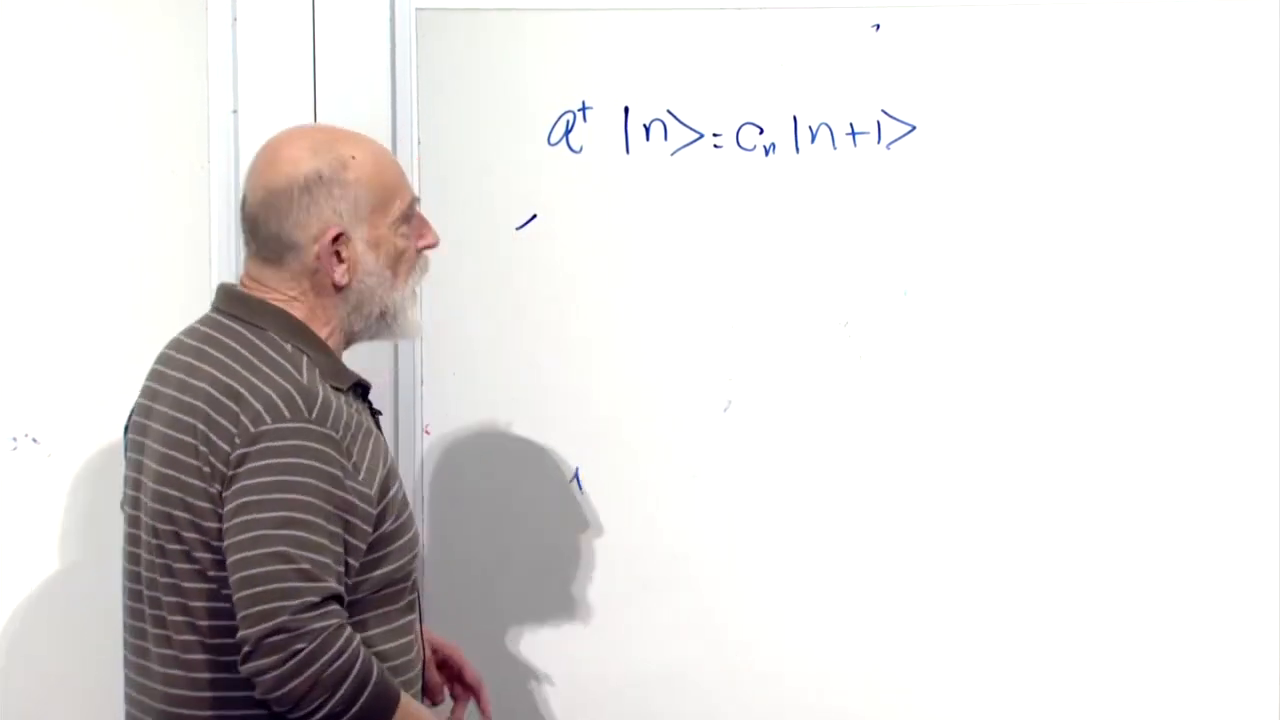
\includegraphics[width=0.9\linewidth]{lecture_06_frame_01.png}
\caption{Der Leiterkoeffizient wird eingeführt, bevor seine Normierung hergeleitet wird. Die Tafelgleichung ist in Gleichung~\eqref{eq:l06-unknown-coefficient} wiedergegeben.}
\lectureframe{00:19:38}
\end{figure}

Wir wählen die Phasenkonvention, in der \(c_n\) reell ist. Hermitesche Konjugation ergibt
\begin{equation}
\langle n|a=c_n\langle n+1|.
\end{equation}
Multipliziert man die beiden Beziehungen und verwendet normierte Basiszustände, so folgt
\begin{align}
c_n^2
&=\langle n|aa^\dagger|n\rangle \\
&=\langle n|(a^\dagger a+1)|n\rangle \\
&=\langle n|(N+1)|n\rangle \\
&=n+1.
\end{align}
Folglich gilt
\begin{equation}
a^\dagger|n\rangle=\sqrt{n+1}\,|n+1\rangle.
\label{eq:l06-raising-rule}
\end{equation}

\begin{classroomqa}
\lecturetimestamp{00:22:35}
\audiencequestion{Warum darf man \(\langle n+1|n+1\rangle=1\) setzen, bevor man \(c_n\) bestimmt?}
\lecturerresponse{Die Eigenvektoren werden von Anfang an als normierte Basis gewählt. Ihre Normierung legt die Normierung von \(a^\dagger|n\rangle\) nicht fest; genau diese noch offene Information steckt im Koeffizienten \(c_n\).}
\end{classroomqa}

Die Regel für den Vernichtungsoperator folgt auf dieselbe Weise:
\begin{equation}
a|n\rangle=\sqrt n\,|n-1\rangle.
\label{eq:l06-lowering-rule}
\end{equation}
Für \(n=0\) verschwindet der Koeffizient automatisch, sodass die Regel auch \(a|0\rangle=0\) einschließt. Bei mehreren Moden verändert der Operator nur die Besetzungszahl in seinem eigenen Eintrag:
\begin{align}
a_i^\dagger|n_1,\ldots,n_i,\ldots\rangle
&=\sqrt{n_i+1}\,|n_1,\ldots,n_i+1,\ldots\rangle, \\
a_i|n_1,\ldots,n_i,\ldots\rangle
&=\sqrt{n_i}\,|n_1,\ldots,n_i-1,\ldots\rangle.
\label{eq:l06-multimode-ladders}
\end{align}
Die übrigen Einträge bleiben unverändert.

\section{Eine Wellenfunktion ist kein Quantenfeld}

Bevor wir ein Feld definieren, müssen wir es von der vertrauten Wellenfunktion unterscheiden. Drei Gegenüberstellungen ordnen den Übergang.

Erstens ist eine Einteilchen-Wellenfunktion
\begin{equation}
\psi(x)=\langle x|\psi\rangle
\end{equation}
eine Darstellung eines Zustandsvektors. Sie ist selbst keine Observable. Wir messen Ort, Impuls, Drehimpuls und weitere Operatoren; die Wellenfunktion liefert die Amplituden, aus denen sich die Wahrscheinlichkeiten dieser Messergebnisse berechnen lassen.

Zweitens hängt eine Vielteilchen-Wellenfunktion von den Orten aller Teilchen ab. Für zwei Teilchen, deren Ortsvektoren vorläufig mit \(x\) und \(y\) bezeichnet seien, gilt
\begin{equation}
\psi(x,y)=\langle x,y|\psi\rangle.
\end{equation}
Hier kennzeichnen \(x\) und \(y\) zwei verschiedene Teilchen; sie sind nicht die kartesischen \(x\)- und \(y\)-Komponenten eines einzigen Ortsvektors. Bei \(N\) Teilchen wird der Zustand dargestellt durch
\begin{equation}
\psi(x_1,x_2,\ldots,x_N).
\end{equation}

Drittens beschreibt diese Wellenfunktion eine feste Teilchenzahl. Eine Wellenfunktion für fünfzehn Teilchen hat fünfzehn Ortsargumente und gehört zu einem Hilbertraum für fünfzehn Teilchen. Für sich allein beschreibt sie keinen Prozess, bei dem sich die Teilchenzahl von fünfzehn auf vierzehn oder sechzehn ändert.

Ein Quantenfeld kehrt diese Merkmale um. Es ist ein Operator statt eines Zustands, hängt von einem räumlichen Punkt \(x\) ab und wirkt auf einen Zustandsraum, der alle Teilchenzahlsektoren enthält. Die Wendung ``ein Punkt'' meint einen frei variierbaren Ortsvektor. Sie bedeutet nicht, dass \(x\) ein einzelner Zahlenwert zugewiesen wurde.

Eine Einschränkung wird später wichtig sein. Das weiter unten eingeführte Feld \(\Psi(x)\) ist nicht hermitesch und daher im strengen Sinn selbst keine Observable. Seine hermiteschen Kombinationen sind Observablen. Die vorläufige Aussage, ein Feld sei messbar, wird also präzisiert und nicht verworfen: Felder sind operatorwertige Funktionen, und ihre hermiteschen Kombinationen stellen messbare Größen dar.

\begin{classroomqa}
\lecturetimestamp{00:36:52}
\audiencequestion{Wenn das Feld eine Funktion des Ortes ist, darf dieser Ort dann variieren? Und was ist aus dem \(y\) in der Zweiteilchen-Wellenfunktion geworden?}
\lecturerresponse{Der Punkt \(x\) durchläuft den gesamten Raum. ``Ein Ort'' bedeutet, dass der Operator ein räumliches Argument hat, nicht dass dieses Argument festliegt. In \(\psi(x,y)\) bezeichnen die Symbole \(x\) und \(y\) die Orte zweier Teilchen; gleichwertig kann man sie als \(x_1\) und \(x_2\) schreiben. Sie sind nicht zwei kartesische Komponenten des Feldarguments.}
\end{classroomqa}

\begin{classroomqa}
\lecturetimestamp{00:38:15}
\audiencequestion{Wie hängen die Beschreibungen durch die Wellenfunktion für feste Teilchenzahl und durch Felder zusammen, und beschreiben sie unterschiedliche Teilchenarten?}
\lecturerresponse{Der Zusammenhang ist die zentrale Konstruktion, die noch aussteht. Es handelt sich um Teilchen derselben Art. In dieser Vorlesung betrachten wir Bosonen; für Fermionen ist eine andere Algebra erforderlich.}
\end{classroomqa}

\section{Ein Teilchen in einem Kasten}

Kehren wir vorübergehend zur gewöhnlichen Einteilchen-Quantenmechanik zurück. Wir bringen ein Teilchen in einem eindimensionalen Kasten unter. Bei nur einem Teilchen ist die Unterscheidung zwischen Boson und Fermion unerheblich: Es gibt kein zweites identisches Teilchen, mit dem man Austausch oder Ausschluss prüfen könnte.

Seien
\begin{equation}
\psi_1(x),\ \psi_2(x),\ \psi_3(x),\ldots
\end{equation}
die Energieeigenfunktionen. Die niedrigste Mode ist die glatteste Welle, die an den Wänden verschwindet. Die nächste Mode hat einen inneren Knoten, und höherenergetische Moden schwingen schneller. Für den idealen unendlich tiefen Potentialkasten der Breite \(L\) ist eine praktische normierte Basis
\begin{equation}
\psi_i(x)=\sqrt{\frac{2}{L}}\sin\!\left(\frac{i\pi x}{L}\right),
\qquad 0<x<L.
\label{eq:l06-box-basis}
\end{equation}
Die explizite Sinusformel ist eine Standardrealisierung der qualitativen Skizze an der Tafel; das folgende Argument erfordert lediglich eine vollständige Orthonormalbasis von Einteilchenzuständen.

\begin{figure}[htbp]
\centering
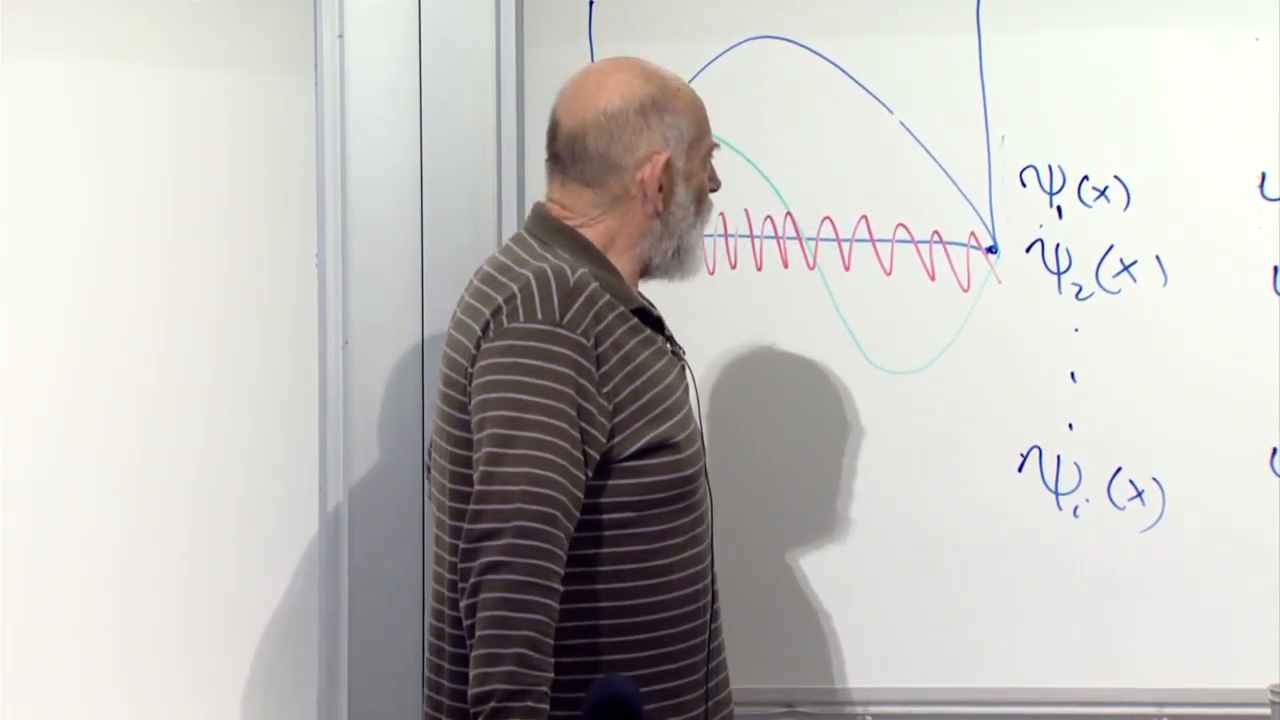
\includegraphics[width=0.9\linewidth]{lecture_06_frame_03.png}
\caption{Einteilchenmoden des Kastens, nach steigender Energie geordnet. Die erste Mode hat keinen inneren Knoten, die zweite einen, und die nicht gezeigten höheren Moden schwingen zunehmend schneller.}
\lectureframe{00:43:10}
\end{figure}

Dieselbe Struktur lässt sich ohne die Verdeckung durch die Live-Tafel neu zeichnen:
\begin{figure}[htbp]
\centering
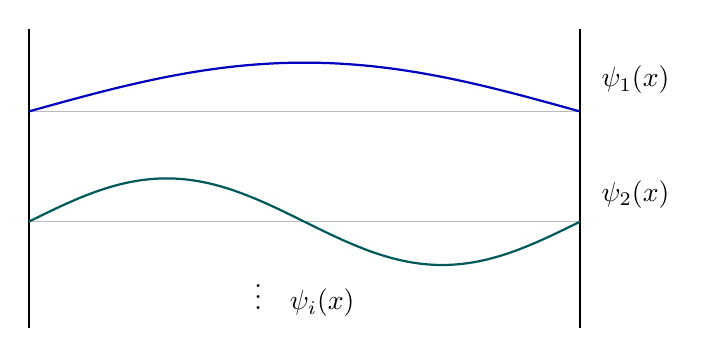
\begin{tikzpicture}[x=1cm,y=1cm]
  \draw[thick] (0,0) -- (0,3.8);
  \draw[thick] (7,0) -- (7,3.8);
  \draw[gray!55] (0,2.75) -- (7,2.75);
  \draw[gray!55] (0,1.35) -- (7,1.35);
  \draw[blue!75!black,thick,domain=0:7,samples=120]
    plot (\x,{2.75+0.62*sin(180*\x/7)});
  \draw[teal!70!black,thick,domain=0:7,samples=120]
    plot (\x,{1.35+0.55*sin(360*\x/7)});
  \node[right] at (7.15,3.15) {$\psi_1(x)$};
  \node[right] at (7.15,1.70) {$\psi_2(x)$};
  \node at (3.5,0.45) {$\vdots\quad \psi_i(x)$};
\end{tikzpicture}
\caption{Eine saubere Rekonstruktion der qualitativen Skizze der Kastenmoden. Die vertikale Verschiebung trennt die Eigenfunktionen zur besseren Lesbarkeit; sie ist keine zusätzliche physikalische Koordinate.}
\end{figure}

Der Index \(i\) kennzeichnet einen Einteilchenzustand, nicht ein Teilchen und auch nicht die Zahl der Knoten. Bei der Kastenbasis ist \(i\) zufällig um eins größer als die Zahl der inneren Knoten. Jeder Zustand hat eine Energie \(\varepsilon_i\). In der Notation der Vorlesung können wir diese Energie als \(\hbar\omega_i\) schreiben oder, nach Setzen von \(\hbar=1\), einfach als \(\omega_i\).

\begin{classroomqa}
\lecturetimestamp{00:39:01}
\audiencequestion{War die frühere Annahme der Unabhängigkeit exakt, und könnte der Index \(i\) die möglichen Zustände eines Elektrons in einem Atom kennzeichnen?}
\lecturerresponse{Für die Konstruktion mit unabhängigen Moden ist die Kommutativität verschiedener Moden exakt. Der Index kann Einteilchenzustände eines Atoms kennzeichnen. Wenn die Teilchen jedoch miteinander wechselwirken, ist der einfache Hamiltonoperator unabhängiger Moden nicht mehr die ganze Beschreibung.}
\end{classroomqa}

\begin{classroomqa}
\lecturetimestamp{00:40:34}
\audiencequestion{Ist das Teilchen im Kasten ein Boson?}
\lecturerresponse{Das kann sein, doch bei einem Teilchen spielt die Statistik keine Rolle. Ausschluss und Austausch werden erst bei mehr als einem identischen Teilchen relevant.}
\end{classroomqa}

\section{Von Kastenmoden zum Fock-Raum}

Lassen wir nun eine beliebige Anzahl identischer Bosonen im Kasten zu. Eine Anzahl \(n_1\) kann \(\psi_1\) besetzen, eine Anzahl \(n_2\) kann \(\psi_2\) besetzen und so weiter. Ein Basiszustand ist daher
\begin{equation}
|n_1,n_2,n_3,\ldots\rangle.
\end{equation}
Dies ist genau die Notation, die bereits für viele Oszillatoren verwendet wurde. Die Übereinstimmung ist strukturell: Jedem Einteilchenzustand wird ein Oszillator zugeordnet, und die Anregungszahl des Oszillators wird mit der Zahl der Teilchen identifiziert, die diesen Zustand besetzen.

Bosonen sind hier wesentlich, denn jedes \(n_i\) kann eine beliebige nichtnegative ganze Zahl sein. Bei Fermionen kann jeder Einteilchenzustand leer oder einfach besetzt sein, niemals doppelt; daher lässt sich die gewöhnliche Oszillatoralgebra nicht unverändert verwenden.

Die Operatoren lassen sich nun durch ihre Wirkung auf die Besetzungszahlbasis definieren. Der Operator \(a_i^\dagger\) erzeugt ein Teilchen im Einteilchenzustand \(i\); \(a_i\) vernichtet eines:
\begin{align}
a_i^\dagger|n_1,\ldots,n_i,\ldots\rangle
&=\sqrt{n_i+1}\,|n_1,\ldots,n_i+1,\ldots\rangle, \\
a_i|n_1,\ldots,n_i,\ldots\rangle
&=\sqrt{n_i}\,|n_1,\ldots,n_i-1,\ldots\rangle.
\end{align}
Das ist keine nachträglich eingeführte Analogie. So sind die bosonischen Erzeugungs- und Vernichtungsoperatoren auf dieser Basis definiert. Da die Basis den Raum aufspannt, legt die Definition durch Linearität ihre Wirkung auf jeden Zustand fest.

\begin{classroomqa}
\lecturetimestamp{00:47:11}
\audiencequestion{Sind \(n_1,n_2,n_3\) die Quantenzustände?}
\lecturerresponse{Die Bezeichnungen \(1,2,3,\ldots\) kennzeichnen die Einteilchenzustände. Die Symbole \(n_1,n_2,n_3,\ldots\) geben die Anzahl der Teilchen an, die diese Zustände besetzen. Die Unterscheidung zwischen Zustandsbezeichnung und zugehöriger Besetzungszahl im Blick zu behalten, ist die wichtigste Notationsaufgabe.}
\end{classroomqa}

\subsection{Was die Quadratwurzel bewirkt}

Der Faktor \(\sqrt{n_i+1}\) steht weder für ein zusätzliches Teilchen noch für einen eigenen physikalischen Prozess. Er sorgt für die richtige Normierung und Algebra des Operators. Für eine Mode gilt
\begin{align}
a a^\dagger|n\rangle
&=a\bigl(\sqrt{n+1}\,|n+1\rangle\bigr) \\
&=(n+1)|n\rangle,
\end{align}
während
\begin{equation}
a^\dagger a|n\rangle=n|n\rangle.
\end{equation}
Ihre Differenz ist daher \(|n\rangle\), wie es \([a,a^\dagger]=1\) verlangt. Die beiden Leiteroperatoren sind grob gesprochen jeweils von der Größenordnung \(\sqrt n\), denn ihr Produkt ergibt den Zahloperator, der von der Größenordnung \(n\) ist.

\begin{classroomqa}
\lecturetimestamp{00:47:52}
\audiencequestion{Welche konkrete physikalische Bedeutung hat der Quadratwurzelfaktor?}
\lecturerresponse{Er dient in erster Linie der mathematischen Normierung. Er stellt sicher, dass die Besetzungszustände normiert sind, dass \(a^\dagger a\) den Eigenwert \(n\) hat und dass die Leiteroperatoren den Oszillatorkommutator erfüllen. Manchmal ist die Mathematik selbst die Bedeutung, die man braucht.}
\end{classroomqa}

\begin{classroomqa}
\lecturetimestamp{00:52:25}
\audiencequestion{Sind die Erzeugungs- und Vernichtungsoperatoren allein durch ihre Eigenschaften und ihre Wirkung auf die Basis definiert worden?}
\lecturerresponse{Ja. Definitionen müssen nicht aus einem grundlegenderen Bild hervorgehen. Ihr Wert zeigt sich an ihren Konsequenzen. Definiert man die Wirkung auf einer vollständigen Basis, sind die Operatoren überall festgelegt, und diese Definitionen reproduzieren die gewünschten Kommutationsrelationen.}
\end{classroomqa}

\begin{classroomqa}
\lecturetimestamp{00:53:22}
\audiencequestion{Warum lässt \(a_i\) ein Teilchen verschwinden, statt es lediglich in einen anderen Zustand zu versetzen?}
\lecturerresponse{Denn \(a_i\) ist so definiert, dass es die Besetzung des Zustands \(i\) erniedrigt. Die nützlichere Frage ist nicht, warum eine Definition gilt, sondern warum sie nützlich ist. Sie ist nützlich, weil Emission und Absorption Operatoren erfordern, die die Teilchenzahl ändern: Bei der Emission von Strahlung wird ein Photon erzeugt, bei seiner Absorption wird es vernichtet.}
\end{classroomqa}

Der von allen Besetzungszahlzuständen aufgespannte Raum heißt \emph{Fock-Raum}. Er enthält das Vakuum, jeden Einteilchenzustand, jeden Zweiteilchenzustand und so weiter, ohne feste obere Grenze:
\begin{equation}
\mathcal F=\mathcal H_0\oplus\mathcal H_1\oplus\mathcal H_2\oplus\cdots.
\label{eq:l06-fock-space}
\end{equation}
Die Direktsummenschreibweise macht explizit, was die gewöhnliche Wellenfunktion für \(N\) Teilchen nicht ausdrückte: Alle Teilchenzahlsektoren gehören zu einem einzigen Zustandsraum.

\begin{classroomqa}
\lecturetimestamp{00:54:56}
\audiencequestion{Legen Definitionen der Operatoren auf den Besetzungszahl-Eigenvektoren ihre Wirkung auf beliebigen Vektoren fest, und folgen daraus die Oszillatorkommutatoren?}
\lecturerresponse{Genau. Die Besetzungsvektoren bilden eine Basis, sodass die Linearität die Definition auf den gesamten Fock-Raum erweitert. Die bosonischen Kommutationsrelationen lassen sich durch Anwendung auf diese Basis überprüfen. Jeder Einteilchenzustand entspricht einem Oszillator, dessen Besetzungszahl der Teilchenzahl in diesem Zustand entspricht.}
\end{classroomqa}

\subsection{Das Vakuum und der freie Hamiltonoperator}

Das Fock-Vakuum ist der Zustand, in dem kein Einteilchenzustand besetzt ist:
\begin{equation}
|0\rangle=|0,0,0,\ldots\rangle,
\qquad a_i|0\rangle=0.
\end{equation}
Der Ausdruck \emph{Grundzustand} kann hier irreführend sein. Der niedrigste \emph{Einteilchen}zustand ist die Mode \(i=1\); im Fock-Vakuum befindet sich jedoch nicht einmal in dieser Mode ein Teilchen. Besetzt ein Teilchen die niedrigste Mode, kann \(a_1\) es entfernen und das System ins Vakuum zurückführen.

\begin{classroomqa}
\lecturetimestamp{00:56:19}
\audiencequestion{Was ist das Vakuum in der Besetzungszahldarstellung? Ist der niedrigste Einteilchenzustand besetzt?}
\lecturerresponse{Im Vakuum sind alle Besetzungszahlen null, und jeder Operator \(a_i\) vernichtet es. Die niedrigste Einteilchenmode ist im Vakuum unbesetzt. Wäre sie besetzt, könnte ihr Vernichtungsoperator das Teilchen entfernen.}
\end{classroomqa}

Für nicht wechselwirkende Teilchen ist die Gesamtenergie additiv. Hat ein Teilchen im Zustand \(i\) die Energie \(\hbar\omega_i\), dann gilt
\begin{align}
H
&=\sum_i \hbar\omega_i N_i \\
&=\sum_i \hbar\omega_i a_i^\dagger a_i.
\label{eq:l06-free-fock-hamiltonian}
\end{align}
Es gibt zwei gleichwertige Lesarten. Der Ausdruck ist die Summe der Oszillatorenergien, mit einem Oszillator pro Einteilchenzustand. Zugleich ist er die Summe der Einteilchenenergien, jeweils multipliziert mit der Zahl der Teilchen, die diese Energie haben.

In der Feldtheorie-Notation heißt \(a_i^\dagger\) üblicherweise Erzeugungsoperator und \(a_i\) Vernichtungsoperator. Die ältere Notation \(a_+\) und \(a_-\) bezeichnet dasselbe.

\section{Klarstellungen vor der Einführung des Feldes}

Mehrere Fragen nach der Pause grenzen die neue Oszillator-Buchhaltung von einem gewöhnlichen Teilchen ab, das sich in einem Oszillatorpotential bewegt.

\begin{classroomqa}
\lecturetimestamp{01:06:09}
\audiencequestion{Die Energieniveaus eines Teilchens im Kasten sind nicht äquidistant. Wo kommt also der harmonische Oszillator ins Spiel?}
\lecturerresponse{Die Einteilchenenergien \(\omega_i\) müssen nicht äquidistant sein. Für jede feste Mode \(i\) sind die Energien von null, einem, zwei und drei nicht wechselwirkenden Teilchen in dieser Mode jedoch \(0,\omega_i,2\omega_i,3\omega_i\). Diese Besetzungsleiter ist der Oszillator. Sie ist davon zu unterscheiden, ein einzelnes Teilchen in ein harmonisches Oszillatorpotential zu setzen.}
\end{classroomqa}

\begin{classroomqa}
\lecturetimestamp{01:08:38}
\audiencequestion{Hängt diese Konstruktion mit der Fourierzerlegung zusammen?}
\lecturerresponse{Auf grundlegende Weise. Besteht die Einteilchenbasis aus Impulsmoden, sind die Modenfunktionen Sinus- und Kosinusfunktionen oder komplexe Exponentialfunktionen, und die \(a_i\) sind quantenmechanische Analoga der Fourierkoeffizienten. Eine allgemeine Basis muss nicht trigonometrisch sein, doch die Logik der Entwicklung ist dieselbe.}
\end{classroomqa}

\begin{classroomqa}
\lecturetimestamp{01:09:07}
\audiencequestion{Wird allen Teilchen dieselbe Energie zugewiesen, und sind Wechselwirkungen eingeschlossen?}
\lecturerresponse{Teilchen im selben Einteilchenzustand haben dieselbe Energie, während Teilchen in verschiedenen Zuständen im Allgemeinen unterschiedliche Energien haben. Vorerst sind die Teilchen frei, sie wechselwirken also nicht. Wechselwirkungen würden zusätzliche potenzielle Energieterme hinzufügen, sodass der Hamiltonoperator nicht mehr nur die additive Summe aus Gleichung~\eqref{eq:l06-free-fock-hamiltonian} wäre.}
\end{classroomqa}

\begin{classroomqa}
\lecturetimestamp{01:10:26}
\audiencequestion{Was ist aus dem halben Quant der Nullpunktsenergie in jedem Oszillator geworden?}
\lecturerresponse{Es ist eine additive Konstante im Hamiltonoperator. Eine Konstante kommutiert mit jedem Operator und verändert daher nicht die Heisenberg-Bewegungsgleichungen; gewöhnliche nichtgravitative Messungen hängen von Energiedifferenzen ab. Für besondere Zwecke kann sie eine Rolle spielen, doch die hier entwickelte Konstruktion wird von ihr nicht beeinflusst.}
\end{classroomqa}

Die freie Theorie ist bereits ein Buchhaltungsinstrument von ungewöhnlicher Leistungsfähigkeit. Sie erfasst nicht nur viele Teilchen, sondern auch Teilchen, die ihren Zustand ändern, entstehen, verschwinden oder in Superpositionen mit unterschiedlicher Gesamtteilchenzahl vorliegen. Die Operatoren sind mehr als bloße Buchhaltungssymbole, denn geeignete hermitesche Kombinationen können gemessen werden; die Buchhaltung ist jedoch eine nützliche erste Anschauung.

\begin{classroomqa}
\lecturetimestamp{01:14:03}
\audiencequestion{Wie sind Feldtheorie und Quantenfeldtheorie historisch entstanden?}
\lecturerresponse{Ein kurzer historischer Abriss beginnt mit Faradays physikalischem Bild elektrischer und magnetischer Felder und Maxwells Gleichungen für klassische Felder. Planck führte bei der Untersuchung der Wärmestrahlung Energiequanten ein; Einstein setzte die Quantisierung mit dem elektromagnetischen Feld selbst und mit Lichtquanten in Verbindung. Heisenberg, Pauli und insbesondere Dirac trugen dann gegen Ende der 1920er-Jahre dazu bei, den modernen Operatorformalismus zusammenzufügen. Die Ultraviolettkatastrophe und die quantenmechanische Beschreibung der Strahlung gehörten zu den entscheidenden frühen Problemen. Dies ist ein schematischer Abriss und keine vollständige Zuweisung von Prioritäten.}
\end{classroomqa}

Der historische Zusammenhang erklärt auch, warum Oszillatoren immer wieder auftreten. Klassische Strahlung in einem Hohlraum lässt sich in Normalmoden zerlegen. Quantisiert man diese Moden, werden ihre Anregungszahlen zu Photonenzahlen. Die mathematischen Quanten, die die Moden besetzen, werden zu physikalischen Teilchen.

\section{Der bosonische Feldoperator}

Sei \(\{\psi_i(x)\}\) eine vollständige Orthonormalbasis von Einteilchen-Wellenfunktionen. Wir definieren
\begin{equation}
\boxed{\Psi(x)=\sum_i a_i\,\psi_i(x)}
\label{eq:l06-field-annihilation}
\end{equation}
und ihren hermitesch konjugierten Operator
\begin{equation}
\boxed{\Psi^\dagger(x)=\sum_i a_i^\dagger\,\psi_i^*(x)}.
\label{eq:l06-field-creation}
\end{equation}

\begin{figure}[htbp]
\centering
\includegraphics[width=0.9\linewidth]{lecture_06_frame_04.png}
\caption{Die vollständigen Modenentwicklungen des Vernichtungsfeldes und seines hermitesch konjugierten Feldes. Die Gleichungen~\eqref{eq:l06-field-annihilation} und \eqref{eq:l06-field-creation} bewahren in gesetzter Form dieselbe Operator- und Komplexkonjugationsstruktur.}
\lectureframe{01:25:15}
\end{figure}

Für einen festen Ort \(x\) ist jedes \(\psi_i(x)\) eine gewöhnliche komplexe Zahl. Der gesamte Operatorgehalt steckt in \(a_i\) und \(a_i^\dagger\). Wenn \(x\) variiert, erhalten wir an jedem Raumpunkt einen anderen Operator. Genau das bedeutet es, dass \(\Psi\) eine operatorwertige Funktion ist.

Sind die Basisfunktionen ebene Wellen, dann sind Gleichungen~\eqref{eq:l06-field-annihilation} und \eqref{eq:l06-field-creation} quantenmechanische Fourierentwicklungen: Die klassischen Fourierkoeffizienten sind zu Operatoren geworden. In einem Kasten kann die Basis stattdessen aus den Sinusfunktionen in Gleichung~\eqref{eq:l06-box-basis} bestehen. Jede vollständige Orthonormalbasis von Einteilchenzuständen ist geeignet.

Weder \(\Psi\) noch \(\Psi^\dagger\) ist hermitesch. Observable Felder lassen sich aus hermiteschen Kombinationen wie
\begin{equation}
\Psi(x)+\Psi^\dagger(x),
\qquad
i\bigl(\Psi^\dagger(x)-\Psi(x)\bigr),
\end{equation}
bilden; observable Dichten werden später aus Produkten wie \(\Psi^\dagger(x)\Psi(x)\) konstruiert. Zunächst geht es darum zu verstehen, was die beiden grundlegenden Felder bewirken.

\begin{classroomqa}
\lecturetimestamp{01:23:14}
\audiencequestion{Wie kann die linke Seite ein Operator sein, wenn die Modenfunktionen rechts gewöhnliche Wellenfunktionen sind?}
\lecturerresponse{Bei festem \(x\) sind die Funktionen \(\psi_i(x)\) Zahlen. Die Faktoren \(a_i\) sind Operatoren. Eine Zahl mal einem Operator ergibt einen Operator, also ist auch die Summe ein Operator. Wenn \(x\) variiert, erhalten wir die ganze Operatorfamilie.}
\end{classroomqa}

\section{Was das Feld bewirkt}

Das Vernichtungsfeld vernichtet das Vakuum unmittelbar:
\begin{equation}
\Psi(x)|0\rangle
=\sum_i\psi_i(x)a_i|0\rangle
=0.
\label{eq:l06-field-kills-vacuum}
\end{equation}
Das Erzeugungsfeld ist aufschlussreicher.

Sei \(|i\rangle\) der Einteilchenzustand mit der Wellenfunktion
\begin{equation}
\langle x|i\rangle=\psi_i(x).
\end{equation}
Die Vollständigkeit der Einteilchenbasis liefert
\begin{equation}
\sum_i|i\rangle\langle i|=1.
\label{eq:l06-completeness}
\end{equation}
Wenden wir diese Identität auf einen Ortseigenzustand an:
\begin{align}
|x\rangle
&=\sum_i|i\rangle\langle i|x\rangle \\
&=\sum_i\psi_i^*(x)|i\rangle.
\label{eq:l06-position-expansion}
\end{align}
In der Fock-Darstellung lautet ein Einteilchen-Modenzustand
\begin{equation}
|i\rangle=a_i^\dagger|0\rangle.
\end{equation}
Setzen wir dies in Gleichung~\eqref{eq:l06-position-expansion} ein, so erhalten wir
\begin{align}
|x\rangle
&=\sum_i\psi_i^*(x)a_i^\dagger|0\rangle \\
&=\Psi^\dagger(x)|0\rangle.
\label{eq:l06-local-creation}
\end{align}
Damit erzeugt \(\Psi^\dagger(x)\) ein bei \(x\) lokalisiertes Teilchen, während \(\Psi(x)\) dort eines vernichtet. Ein Ortseigenzustand ist deltaförmig lokalisiert und ein verallgemeinerter, nicht normierbarer Zustand; ein physikalisch lokalisiertes Teilchen erhält man, indem man das Feld mit einem normierbaren Wellenpaket verschmiert.\editorialnote{Die Vorlesung verwendet die idealisierte Sprache der Ortseigenzustände. Die Ergänzung zum Wellenpaket hält die mathematische Standardbedeutung fest, ohne das Argument zu verändern.}

\begin{classroomqa}
\lecturetimestamp{01:36:26}
\audiencequestion{Wo steckt die Information darüber, welche Teilchenart erzeugt wird? Ist der Zustand bei \(x\) deltaförmig lokalisiert?}
\lecturerresponse{Jeder Teilchensorte wird ein eigenes Feld zugeordnet; die Identität des Teilchens ergibt sich also daraus, welches Feld verwendet wird. Das Argument \(x\) legt fest, wo es erzeugt wird. In der idealisierten Ortsbasis ist der erzeugte Zustand deltaförmig lokalisiert.}
\end{classroomqa}

Beispiele für Bosonensorten sind Photonen, Gravitonen, Higgs-Bosonen und Gluonen, doch realistische Felder tragen auch innere Indizes. Selbst Photonen benötigen Polarisationsindizes. Die vereinfachte Notation für ein skalares Feld lässt diese zusätzlichen Indizes weg, damit das Erzeugungsprinzip sichtbar bleibt.

\subsection{Das Vakuum ist nicht der Nullvektor}

Die Gleichung
\begin{equation}
\Psi(x)|0\rangle=0
\end{equation}
enthält zwei sehr verschiedene Objekte, die mit null bezeichnet werden. Der Ket \(|0\rangle\) ist das Vakuum: ein normierter physikalischer Zustand mit
\begin{equation}
\langle0|0\rangle=1.
\end{equation}
Das Ergebnis auf der rechten Seite ist der Nullvektor. Seine Norm ist null; er kann nicht normiert werden und stellt keinen physikalischen Zustand dar.

Der Unterschied wird bei der Addition deutlich. Addiert man den Nullvektor zu einem Einteilchenzustand, ändert sich nichts. Addiert man das Vakuum zu einem Einteilchenzustand, erhält man eine echte Superposition verschiedener Teilchenzahlsektoren. Mit normierten Koeffizienten
\begin{equation}
|\chi\rangle=\frac{1}{\sqrt2}\bigl(|0\rangle+|1\rangle\bigr)
\end{equation}
hat die Superposition gleiche Wahrscheinlichkeiten für null und ein Teilchen. Sie ist nicht dasselbe wie \(|1\rangle\).

\begin{classroomqa}
\lecturetimestamp{01:37:23}
\audiencequestion{Wenn bei \(x\) kein Teilchen vorhanden ist, bewirkt \(\Psi(x)\) dann einfach nichts? Was bedeutet es, dass das Ergebnis null ist?}
\lecturerresponse{Sie gibt nicht den ursprünglichen Zustand zurück, sondern den Nullvektor. Das Vakuum ist ein normierter Zustand, der den leeren Raum beschreibt; der Nullvektor hat die Länge null und beschreibt keinen physikalischen Zustand. Jeder Operator, der auf den Nullvektor wirkt, gibt den Nullvektor zurück.}
\end{classroomqa}

\begin{classroomqa}
\lecturetimestamp{01:39:00}
\audiencequestion{Was geschieht, wenn man statt des Nullvektors das Vakuum zu einem Einteilchenzustand addiert?}
\lecturerresponse{Man erhält eine Superposition mit Amplituden für verschiedene Teilchenzahlen. Addiert man dagegen den Nullvektor, bleibt der Einteilchenzustand unverändert. Das Symbol \(|0\rangle\) steht für die Besetzungszahl null; es bedeutet nicht Nullvektor.}
\end{classroomqa}

\begin{classroomqa}
\lecturetimestamp{01:41:56}
\audiencequestion{Spielt es in der Feldentwicklung eine Rolle, in welcher Reihenfolge eine Modenfunktion und ihr Erzeugungs- oder Vernichtungsoperator stehen? Können die Modenfunktionen komplex sein?}
\lecturerresponse{Die Modenfunktion ist eine gewöhnliche Zahl und kommutiert daher mit jedem Operator; die Reihenfolge spielt also keine Rolle. Im Allgemeinen können die Modenfunktionen komplex sein. Ob eine gewählte Basis reell oder komplex ist, hängt vom jeweiligen Einteilchen-Schr\"odinger-Problem ab.}
\end{classroomqa}

\subsection{Zwei Teilchen und die Entstehung bosonischer Symmetrie}

Um ein Teilchen bei \(x\) und ein weiteres bei \(y\) zu erzeugen, wenden wir den Erzeugungsoperator zweimal an:
\begin{equation}
|x,y\rangle
=\Psi^\dagger(y)\Psi^\dagger(x)|0\rangle.
\label{eq:l06-two-particle-state}
\end{equation}
Die Punkte können zusammenfallen oder verschieden sein. Da die zugrunde liegenden Erzeugungsoperatoren kommutieren, gilt
\begin{align}
[\Psi^\dagger(x),\Psi^\dagger(y)]
&=\sum_{i,j}\psi_i^*(x)\psi_j^*(y)
[a_i^\dagger,a_j^\dagger] \\
&=0.
\end{align}
Daraus folgt
\begin{equation}
\Psi^\dagger(y)\Psi^\dagger(x)|0\rangle
=\Psi^\dagger(x)\Psi^\dagger(y)|0\rangle.
\label{eq:l06-boson-exchange}
\end{equation}
Die Reihenfolge der beiden Teilchen zu vertauschen, ändert nichts. Das ist genau die bosonische Austauschsymmetrie. Wir hätten daher auch von der Oszillatoralgebra ausgehen und \emph{ableiten} können, dass Teilchen, die mit kommutierenden Erzeugungsoperatoren konstruiert werden, Bosonen sind. Für Fermionen werden stattdessen antikommutierende Operatoren benötigt.

\begin{classroomqa}
\lecturetimestamp{01:42:37}
\audiencequestion{Wie fügt man dem Einteilchenzustand ein zweites Teilchen hinzu?}
\lecturerresponse{Man wendet ein weiteres Erzeugungsfeld an. Um ein Teilchen bei \(y\) hinzuzufügen, wirkt man mit \(\Psi^\dagger(y)\) von links auf \(\Psi^\dagger(x)\). Das Ergebnis ist der Zweiteilchenzustand aus Gleichung~\eqref{eq:l06-two-particle-state}.}
\end{classroomqa}

\begin{classroomqa}
\lecturetimestamp{01:46:04}
\audiencequestion{Ist die Kommutativität der beiden Erzeugungsfelder vollständig gleichbedeutend damit, den Zweiteilchenzustand zu symmetrisieren?}
\lecturerresponse{Ja. Dadurch ist der Zustand mit einem Teilchen bei \(x\) und einem bei \(y\) identisch mit dem Zustand, der durch Vertauschen der Bezeichnungen entsteht. Das ist die definierende Austauscheigenschaft identischer Bosonen.}
\end{classroomqa}

\begin{classroomqa}
\lecturetimestamp{01:46:32}
\audiencequestion{Bedeutet das, dass die Teilchen bei \(x\) und \(y\) von derselben Bosonenart sein müssen?}
\lecturerresponse{Ja. Die Argumente \(x\) und \(y\) bezeichnen Positionen, während ein Feld eine Teilchensorte beschreibt. Für verschiedene Sorten und zusätzliche Bezeichnungen wie die beiden Polarisationen des Photons sind unterschiedliche Feldkomponenten erforderlich.}
\end{classroomqa}

\section{Warum eine veränderliche Teilchenzahl wichtig ist}

Enthielte ein Problem für alle Zeiten genau 37 Teilchen, wäre die Feldsprache eine optionale Buchführung. Ihre eigentliche Stärke zeigt sich, wenn Teilchen emittiert und absorbiert werden können, insbesondere aber dann, wenn die Teilchenzahl selbst eine quantenmechanische Variable ist. Der Fock-Raum erlaubt Zustände der Form
\begin{equation}
|\Phi\rangle
=c_0|0\rangle+c_1|1\rangle+c_2|2\rangle+\cdots,
\qquad
\sum_{n=0}^{\infty}|c_n|^2=1.
\end{equation}
Ein Laserfeld ist ein wichtiges Beispiel: Im Allgemeinen ist es kein Zustand mit einer exakt festgelegten Photonenzahl, sondern eine Superposition aus vielen Teilchenzahlsektoren.

Die Verbindung zwischen Teilchen und Feldern ist nun explizit. Die Modenoperatoren zählen Teilchen in Energieeigenzuständen und verändern ihre Zahl; das Feld kombiniert diese Operatoren mit einem vollständigen Satz von Wellenfunktionen, sodass Teilchen an bestimmten Positionen erzeugt oder vernichtet werden können. Die Algebra harmonischer Oszillatoren ist zur elementaren Sprache eines bosonischen Quantenfeldes geworden.